\documentclass[]{IEEEtran}

% Your packages go here
\usepackage[utf8]{inputenc}
\usepackage{graphicx}

\markboth{MC949/MO446 Computer Vision}{}

\begin{document}
  \title{Homework 0}
  \author{Leonardo Rezende, Thales Oliveira (RA 148051) and Iury Cleveston (RA 230216)
    \thanks{-, t148051@dac.unicamp.br, iurycl@gmail.com}
  }
  \maketitle
  
  \begin{abstract}
    In this project the group was able to get in contact with the development environment to be worked with during the Computer Vision Course. The exercises proposed were completed, and the manipulated images are shown throughout this report. By resolving the problems, the group was able to work with OpenCV and related libraries for image manipulation in the Python programming language.
  \end{abstract}
  
  \section{Introduction}
  
  This work, developed by Group 8 of Computer Vision Course (2nd Semester/2019), has the objective of introducing the tools used in the field of Computer Vision, and also to practice programming skills needed to succeed in the following projects. The theme of the exercises is basic image manipulation using OpenCV library, and the group decided to work with the Python programming language. The project consists of 5 exercises, divided by specific parts. The solutions of each question, which can be output images, text answers or both, are listed in the next section (Image outputs and Answers). The Conclusion section sums up the work done. 


  \section{Image outputs and Answers}
  \subsection{Exercise 1}
  For this exercise, it was supposed to find an image to be used as input for the next exercises. The chosen image is displayed in figure \ref{fig:i-1-0}, and it is 300x400 pixels, in order to fit the requirements.
  \begin{figure}[!h]
    \centering
    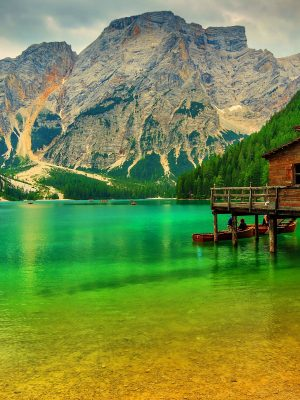
\includegraphics[width=0.8\hsize]{../input/i-1-0.jpg}
    \caption{Image input used for exercises 2 to 5}
    \label{fig:i-1-0}
  \end{figure}

  actions and work goes here.
  
  
  
  \subsection{Exercise 2}
  
  The first question asked to swap the blue and red channels in the original image. The result can be seen in Figure~\ref{fig:o-2-a-0}.
  
  \begin{figure}[!h]
    \centering
    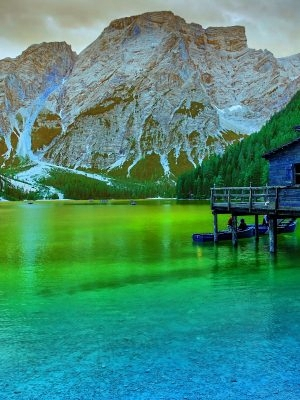
\includegraphics[width=0.8\hsize]{../output/o-2-a-0.jpg}
    \caption{Output image after swapping the blue and red channels.}
    \label{fig:o-2-a-0}
  \end{figure}
  
  In the second question, we should generate a green monochromatic image. This process was executed by selecting the green channel in the original image. The result is presented in Figure~\ref{fig:o-2-b-0}.
  
  \begin{figure}[!h]
    \centering
    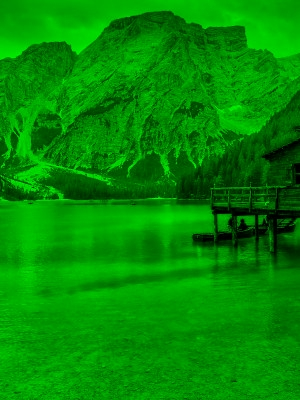
\includegraphics[width=0.8\hsize]{../output/o-2-b-0.jpg}
    \caption{Output image after selecting the green channel.}
    \label{fig:o-2-b-0}
  \end{figure}
  
  In the third question, we should generate a red monochromatic image. This process was executed by selecting the red channel in the original image. The result generated is shown in Figure~\ref{fig:o-2-c-0}.
  
  \begin{figure}[!h]
    \centering
    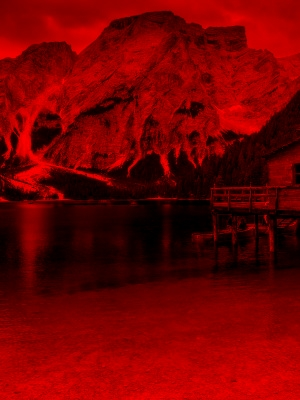
\includegraphics[width=0.8\hsize]{../output/o-2-c-0.jpg}
    \caption{Output image after selecting the red channel.}
    \label{fig:o-2-c-0}
  \end{figure}
  
  The green monochrome image looks better because it holds more information than the red one, which has many areas in dark. The computer vision algorithm should perform better in the green image because the saliency map can be identified easily and the feature description can be more useful.
  
  
  
  \subsection{Exercise 5}
  
  In this exercise, we should take the original colored image and add gaussian noise to the pixels in the green channel. The sigma was defined as 20. The noise increase as the sigma increased. The image seems corrupted as shown in Figure~\ref{fig:o-5-a-0}.
  
  \begin{figure}[!h]
    \centering
    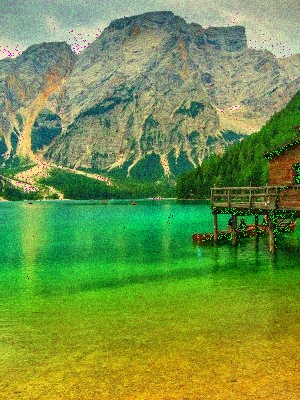
\includegraphics[width=0.8\hsize]{../output/o-5-a-0.jpg}
    \caption{Output image after adding noise to the green channel.}
    \label{fig:o-5-a-0}
  \end{figure}
  
  In the second question, we should the the same gaussian noise the blue channel. The result is shown in Figure~\ref{fig:o-5-b-0}.
  
   \begin{figure}[!h]
    \centering
    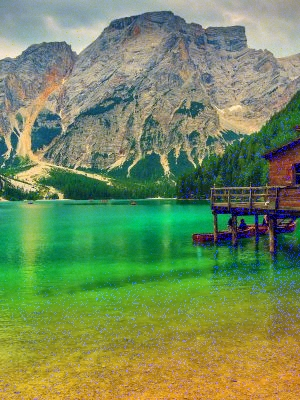
\includegraphics[width=0.8\hsize]{../output/o-5-b-0.jpg}
    \caption{Output image after adding noise to the blue channel.}
    \label{fig:o-5-b-0}
  \end{figure}
  
  The image in which the blue channel received the noise looks better because the blue channel holds less information in terms of saliency and high energy regions than the other channels. So the added noise produced a little impact on the image's content.
  
  
  \section{Conclusion}
  
  You conclude your work here.
  
\end{document}
